\begin{comment}

\subsection{RENEW ROI CRITERION}
%Diagrama2
The $ROI$ is an important element in the algorithm, therefore it will be used
as pattern to find a match of tracked target at the current image. 
The  question in this case is to know the best moment to refresh the $ROI$
with a new perspective of target. 
Here, we establish the criterion that; when the comparison of images return 
a $PCC$ value lower than $0.925$ and greater than $0.8$, then the $ROI$ is changed with the current 
analyzed region and a new position of $ROI$ is with $(x_i,y_i,d_i)$. 
Thus, it was adopted as $0.8$ the lower limit to a match case\cite{Eugene},
see Fig. \ref{fig:newroicri}. Values less than $0.8$ causes a  lost target alert.
Finally, it is important to note that if the $ROI$ is changed, the new $ROI$ is 
the real size of the analyzed region and not with the rescaled version used
in the calculus of the $PCC$.


\begin{figure}[H]
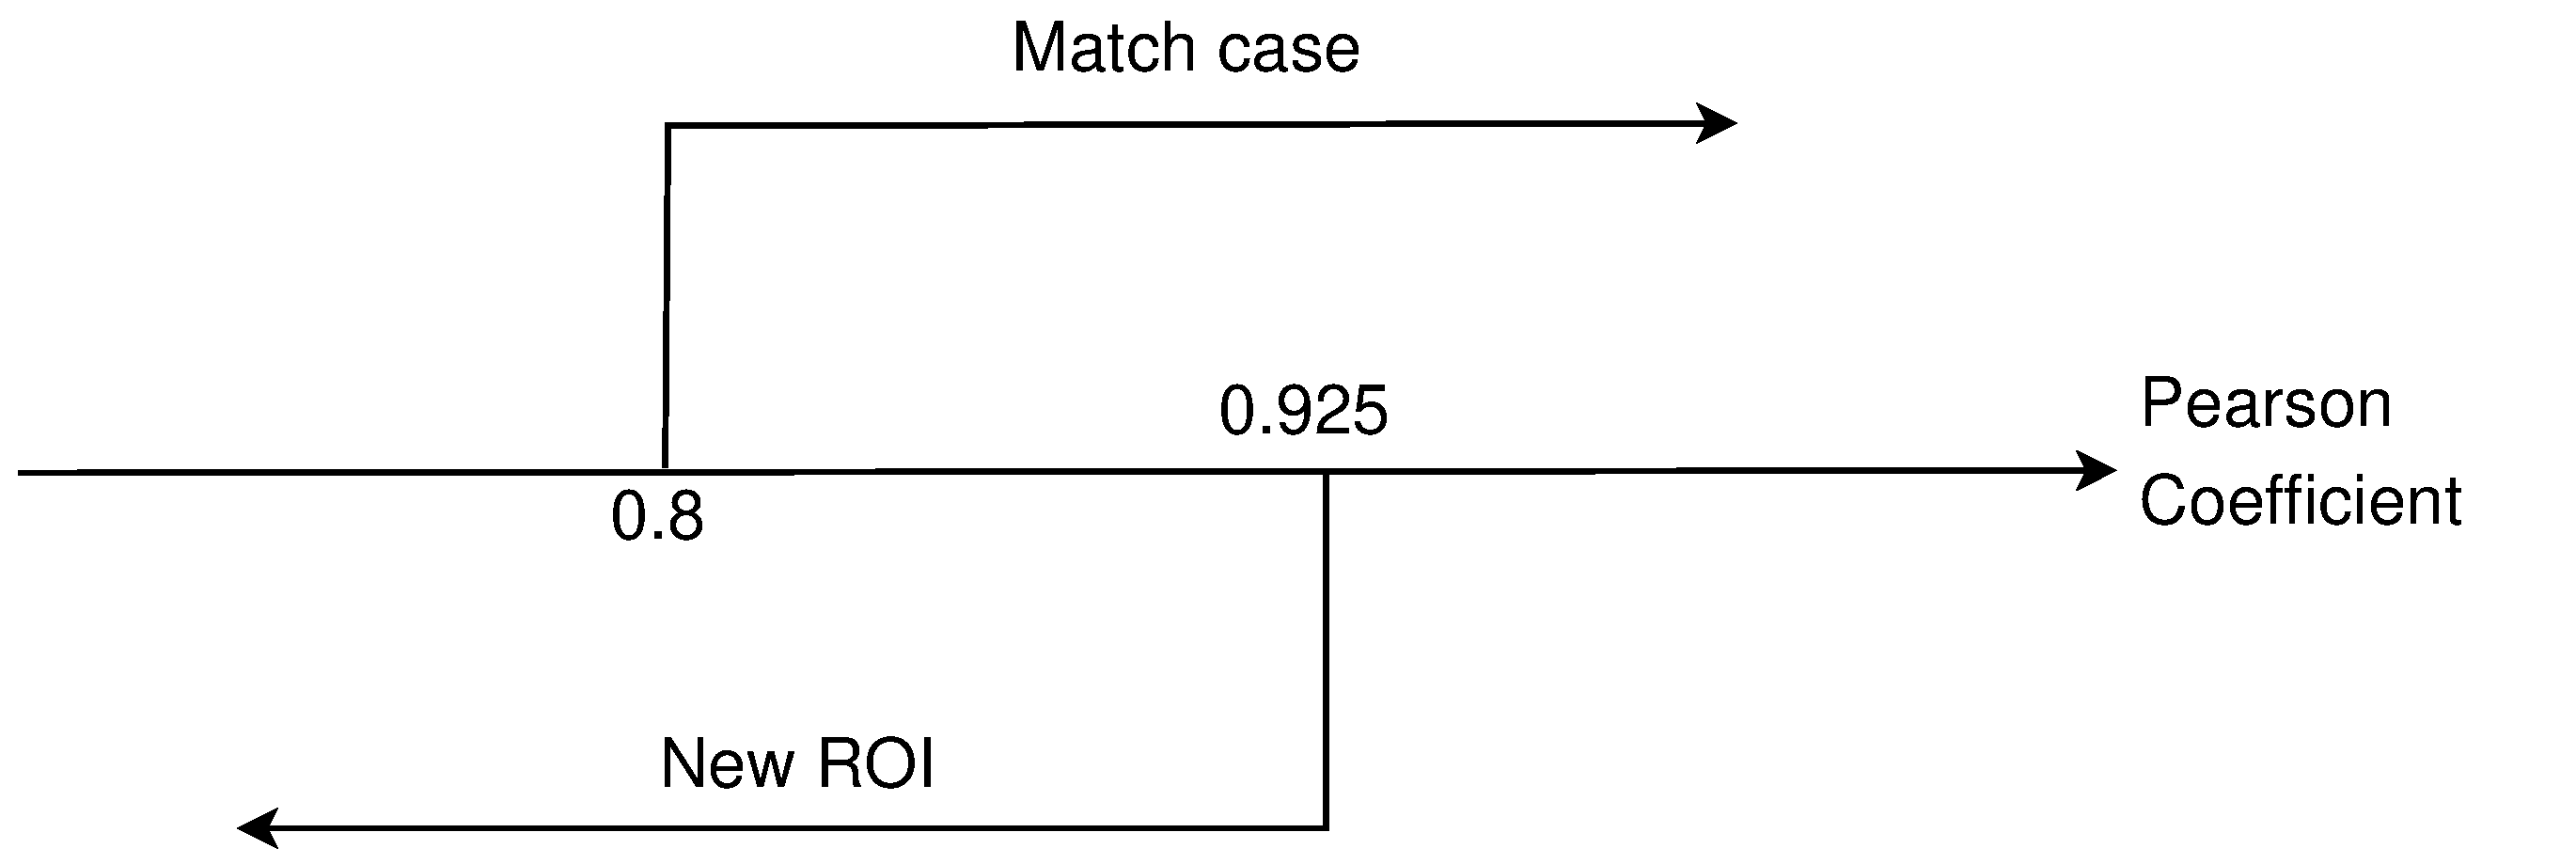
\includegraphics[width=\columnwidth]{images/figure3.eps}
\caption{When the comparison is greater than $0.8$, including numbers bigger than 
$0.925$, it means that the target was matched. But if two regions are compared 
and the $PCC$ is less than $0.925$ and greater than $0.8$, 
then the $ROI$ changes to the current analyzed region.}
\label{fig:newroicri}
\end{figure}

The Algorithm \ref{alg:newroi} shows the criteria described in the
Fig. \ref{fig:newroicri}; the $renew\_roi\_criteria()$ function, explained here,
it is used by the Algorithm \ref{alg:system} of Fig. \ref{fig:system}.

\begin{algorithm}
 \KwData{Initial $ROI$, your position $P_0$, the current matched analysis region ($AR$), your position $P$ and the correlation $r$ between them. }
 \KwResult{The new $ROI$, your position and a status variable, $Found$. }

    $NEWP_0 \leftarrow  P_0$ \;
    $NEWROI \leftarrow  ROI$ \;
    
    \eIf{$0.8 \leq r$}
    {
      $Found \leftarrow True$\;
        message ``target found''\;
        \eIf{$r \leq 0.925$}
        {
            $NEWROI \leftarrow  AR$\;
            $NEWP_0 \leftarrow  P$\;
        }
    }
    {
      message ``target lost''\;
      $Found \leftarrow False$\;
    }
\Return  $\{NEWROI,~NEWP_0,~FOUND\}$\;
\label{alg:newroi}
\caption{$renew\_roi\_criteria(ROI,P_0,AR,P,r)$ function.}
\end{algorithm}
%The system needs to have a high level of reliability, so that the lower limit adopted 
%contributes to an operation with minimum of mistakes.

\end{comment}

%%%%%%%%%%%%%%%%%%%%%%%%%%portugues%%%%%%%%%%%%%%%%%%%%%%%%%%%%%%%%%%%%%%%%%%%%%%%%%%%%%%%



\subsection{Cretério para um novo ROI}

O ROI é um importante elemento dentro algoritmo, pois ele é a referência do
atual estado do objeto que será comparado com as imagens posteriores.
O critério para atualizar o ROI foi determinado a partir da correlação 
entre as imagens, sendo assim, se o valor da comparação estiver entre $0,925$ 
e $0,8$ o ROI será atualizado com uma nova posição $(x_i,y_i,d_i)$.

Deste modo, foi adotado que o limite inferior é de 0,8 \cite{Eugene}. Valores
de comparação abaixo deste, o objeto é tido como perdido, como mostrado na figura
\ref{fig:newroicri}.
Nota-se que o ROI é atualizado para uma escala igual a anterior ou modificada,
dependendo do valor da comparação dada pelo PCC.


\begin{figure}[H]
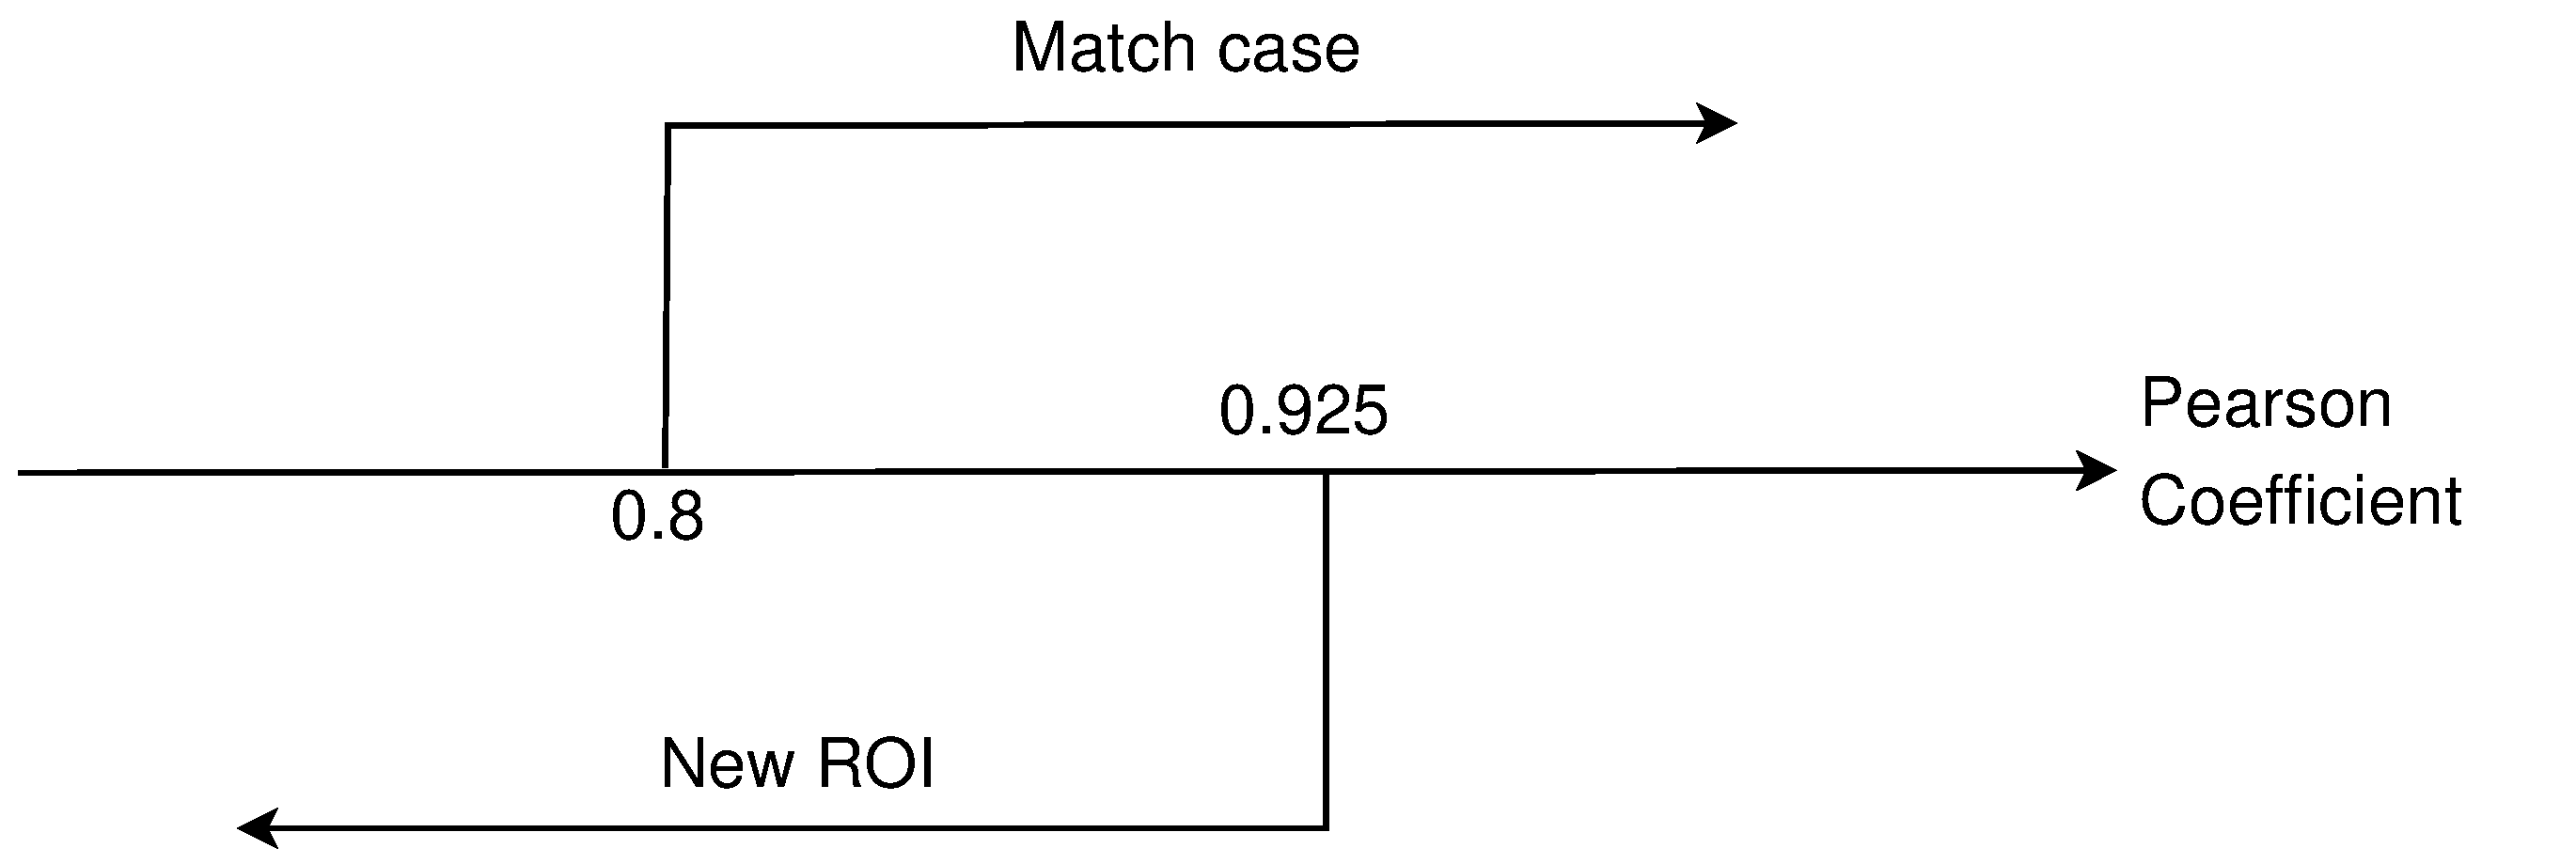
\includegraphics[width=\columnwidth]{images/figure3.eps}
\caption{Quando a comparação é maior que $0,8$, incluindo número maiores que $0,925$, significa que o objeto foi encontrado,
se o PCC é menor que $0,925$ a imagem é tida como perdida e se o coeficiente for maior que $0,8$, então o ROI é atualizado pela imagem de 
maior correlação.}
\label{fig:newroicri}
\end{figure}

O algoritmo \ref{alg:newroi} apresenta o criterio descrito na figura \ref{fig:newroicri};
O função $renew\_roi\_criteria()$ explicada é usada pelo algoritmo \ref{alg:system} da figura \ref{fig:system}


\begin{algorithm}
 \KwData{$ROI$ inicial, posição $P_0$, região de busca do frame atual ($AR$), posição $P$ e a correlação $r$ entre eles. }
 \KwResult{O $ROI$ atualizado, posição e seu status, $Found$. }

    $NEWP_0 \leftarrow  P_0$ \;
    $NEWROI \leftarrow  ROI$ \;
    
    \eIf{$0.8 \leq r$}
    {
      $Found \leftarrow True$\;
        message ``target found''\;
        \If{$r \leq 0.925$}
        {
            $NEWROI \leftarrow  AR$\;
            $NEWP_0 \leftarrow  P$\;
        }
    }
    {
      message ``target lost''\;
      $Found \leftarrow False$\;
    }
\Return  $\{NEWROI,~NEWP_0,~FOUND\}$\;
\label{alg:newroi}
\caption{$renew\_roi\_criteria(ROI,P_0,AR,P,r)$ function.}
\end{algorithm}
%The system needs to have a high level of reliability, so that the lower limit adopted 
%contributes to an operation with minimum of mistakes.
